\documentclass[a4paper, 12pt]{article}%тип документа

%отступы
\usepackage[left=2cm,right=2cm,top=2cm,bottom=3cm,bindingoffset=0cm]{geometry}
\setlength{\parindent}{5ex}

%Русский язык
\usepackage[T2A]{fontenc} %кодировка
\usepackage[utf8]{inputenc} %кодировка исходного кода
\usepackage[english,russian]{babel} %локализация и переносы

%Вставка картинок
\usepackage{graphicx}
\graphicspath{{pictures/}}
\DeclareGraphicsExtensions{.pdf,.png,.jpg}

%Графики
\usepackage{pgfplots}
\pgfplotsset{compat=1.9}

%Математика
\usepackage{amsmath, amsfonts, amssymb, amsthm, mathtools}

%Таблицы
\usepackage{longtable} 
\usepackage{float}

%Римские цифры
\newcommand{\RomanNumeralCaps}[1]{\uppercase\expandafter{\romannumeral#1}}

\usepackage{multirow}


\begin{document}
	\begin{titlepage}
		\begin{center}
			\textsc{Федеральное государственное автономное образовательное учреждение высшего образования«Московский физико-технический институт (национальный исследовательский университет)»\\[5mm]
			}
			
			\vfill
			
			\textbf{Отчёт по лабораторной работы 3.1.3\\[3mm]
				Измерение магнитного поля Земли
				\\[50mm]
			}
			
		\end{center}
		
		\hfill
		\begin{minipage}{.5\textwidth}
			Выполнил студент:\\[2mm]
			Сериков Василий Романович\\[2mm]
			группа: Б03-102\\[5mm]
			
		\end{minipage}
		\vfill
		\begin{center}
			Москва, 2022 г.
		\end{center}
		
	\end{titlepage}
	
	\newpage
	\textbf{Аннотация}\\
	
	
	\textbf{Цель работы: }\\
	
	Определение удельного заряда электрона на основе закона
	«трех вторых» для вакуумного диода.
	
	\textbf{В работе используются: }\\
	
	Вакуумная лампа с цилиндрическим анодом;
	амперметр; многопредельные микроамперметр и вольтметр постоянного
	тока; стабилизированные источники постоянного тока и постоянного напряжения.
	
	
	\textbf{Теоретические сведения: } \\
	
	
	В работе исследуется зависимость величины тока, проходящего через
	вакуумный диод, от напряжения на нём (положительная ветвь вольтамперной характеристики). Наибольший интерес представляет та область значений положительного напряжения на диоде, для которой пространственный заряд (электронное облако) в лампе существенно влияет на распределение электрического поля между катодом и анодом (режим пространственного заряда). Электрическое поле этого заряда «экранирует» поле вблизи катода, из-за чего лишь незначительная часть электронов, способных преодолеть энергетический барьер («работу выхода») и высвобождаемых из катода, создаёт ток через диод. Величина тока в этом режиме пропорциональна напряжению на диоде в степени 3/2.
	
	$$ I \propto  U^{3/2} $$
	
	В данной работе используется диод цилиндрической формы.
	
	Распределение потенциала по радиусу внутри диода определяется уравнением Пуассона в цилиндрических координатах:
	
	\begin{equation}
		\Delta U = \dfrac{d^2U}{dr^2} + \dfrac{1}{r} + \dfrac{dU}{dr} = - \dfrac{\rho(r)}{\varepsilon_0}
	\end{equation}
	
	При этом плотность заряда $ \rho(r) $ связана с текущим через слой диода толщины $ l $ током $ I $ формулой $ I = -2\pi r \rho(r)v(r)l$. При этом из закона сохранения энергии мы находим скорость $ v(r) $ электронов , прошедших через разность потенциалов $ V(r) $: $ \frac{mv^2}{2} = eU(r) $.
	
	\begin{equation}\label{ur}
		r \dfrac{d^2U}{dr^2} + \dfrac{dU}{dr} = \dfrac{I}{2\pi\epsilon_0}\sqrt{\dfrac{m}{2eU}}
	\end{equation}
	
	 В дифференциальном уравнении 2-ого порядка относительно $ U(r) $ нам неизвестен ток I, зависящий от V. Из физических соображений будем полагать:
	
	\begin{equation}
		\dfrac{dU}{dt}\bigg |_{r=r_k} = 0
	\end{equation} 
	
	Наше предположение означает что вблизи катода пространственный заряд электронов полностью экранирует поле анодной разности потенциалов.
	
	Уравнение является нелинейным. Попробуем  найти некое частное решение, где $ U_a = U_{a0}, $ при котором ток $ I = I_0 $. Тогда выражения 
	
	\begin{equation}
		I = I_o \left( \dfrac{U_a}{U{a0}} \right) ^{3/2}, \qquad U(r) = U_{a0}(r)\dfrac{U_a}{U_{a0}}
	\end{equation}
	
	являются решением уравнения, что проверяется подстановкой. В общем виде решение записывается в виде
	
	\begin{equation}
		I = \dfrac{8\sqrt{2}\pi \epsilon_0 l}{9}\sqrt{\dfrac{e}{m}}\dfrac{1}{r_a\beta^2} U^{3/2}
	\end{equation}
	
	Это и есть так называемый "<закон трех вторых"> -- ток в вакуумном диоде пропорционален напряжению на нем в степени 3/2. Он справедлив при любой геометрии электродов, если ток не слишком велик или слишком мал. 
	
	Выпишем в явном виде выражение для удельного заряда:
	
	\begin{equation}
		\frac{e}{m} = \frac{81r_a^2\beta^4}{128\pi^2\varepsilon_0^2l^2}  \frac{I^2}{U^2} = a \frac{I^2}{U^3}
	\end{equation}
	
	\textbf{Экспериментальная установка: }\\
	
	Схема экспериментальной установки изображена на рис. 1. Для питания цепи накала и анода используются два регулируемых источника
	напряжения. Ток накала $I_H$ измеряется амперметром, включённым последовательно с балластным сопротивлением R. Анодное напряжение U
	измеряется вольтметром, анодный ток I — миллиамперметром. В работе
	предлагается измерять анодные токи и напряжения в широком диапазоне значений, перекрывающем примерно три порядка величины, поэтому вольтметр и миллиамперметр должны быть оснащены устройствами ручного или автоматического переключения диапазонов измерения.
	
	\begin{figure}[H]
		\center{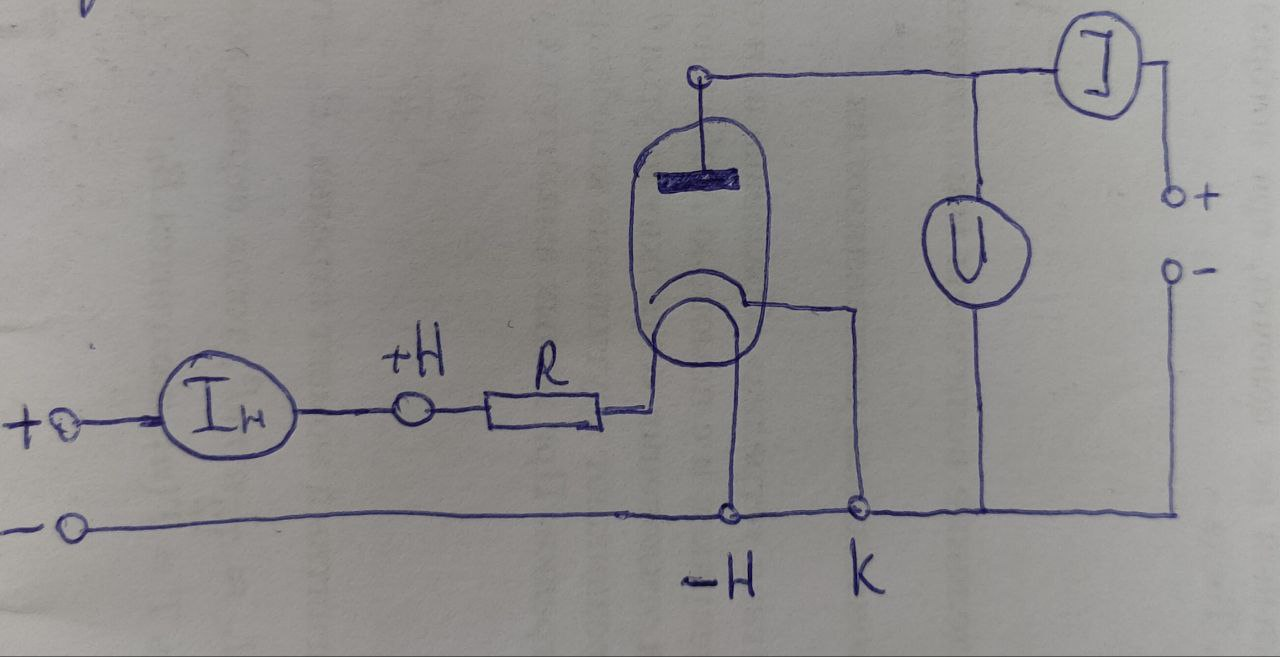
\includegraphics [scale=0.4]{ust.jpeg}}
		\caption{Схема установки.}
	\end{figure}
	
	\newpage
	
	\textbf{Ход работы и обработка результатов: }\\
	
	\begin{enumerate}
	
	\item Проведем подробные измерения вольт-амперных характеристик диода $I(U)$ во всём допустимом диапазоне изменения напряжений (0,5 В - 50 В). Полуученные данные занесем в таблицу 1.
	
	
	\begin{longtable} {|c|c|c|c|c|c|c|c|c|c|}
		\hline
		$I_a$, мкА & 3,5 & 11,4 & 22,8 & 37,2 & 52,6 & 69,8 & 89,5 & 107,3  & 129,1\\ \hline
		$U$, В & 0,5 & 1,0 & 1,5 & 2,0 & 2,5 & 3,0 & 3,5  & 4,0 & 4,5\\ \hline
		\hline
		$I_a$, мкА & 151,5 & 176,4 & 202,0 & 252,8 & 316,0 & 376,6 & 441,5 & 865,0 & 1361,0 \\ \hline
		$U$, В & 5,0 & 5,5 & 6,0 & 7,0 & 8,0 & 9,0 & 10 & 15 & 20\\ \hline
		\hline
		$I_a$, мкА & 1946,0 & 2589,0 & 3279,0 & 4031,0 & 4832,0 & 5776,0 & & &\\ \hline
		$U$, В & 25 & 30 & 35 & 40 & 45 & 50 & & &\\ \hline
		\caption{$I_H = 1,3$ А, $\varepsilon_U = 1\%$, $\varepsilon_{I_a} = 1\%$}
	\end{longtable}
	
	
	\begin{longtable} {|c|c|c|c|c|c|c|c|c|c|}
		\hline
		$I_a$, мкА & 7,3 & 17,4 & 28,6 & 45,4 & 63,0 & 79,8 & 101,0 & 121,6  & 146,2\\ \hline
		$U$, В & 0,5 & 1,0 & 1,5 & 2,0 & 2,5 & 3,0 & 3,5  & 4,0 & 4,5\\ \hline
		\hline
		$I_a$, мкА & 166,8 & 194,3 & 220,1 & 279,0 & 339,2 & 403,8 & 472,9 & 915,5 & 1423,0 \\ \hline
		$U$, В & 5,0 & 5,5 & 6,0 & 7,0 & 8,0 & 9,0 & 10 & 15 & 20\\ \hline
		\hline
		$I_a$, мкА & 2011,0 & 2661,0 & 3374,0 & 4133,0 & 4945,0 & 5897,0 & & &\\ \hline
		$U$, В & 25 & 30 & 35 & 40 & 45 & 50 & & &\\ \hline
		\caption{$I_H = 1,4$ А, $\varepsilon_U = 1\%$, $\varepsilon_{I_a} = 1\%$}
	\end{longtable}
	
	
	\begin{longtable} {|c|c|c|c|c|c|c|c|c|c|}
		\hline
		$I_a$, мкА & 14,0 & 24,4 & 40,6 & 59,1 & 77,7 & 98,1 & 118,6 & 142,0 & 166,0\\ \hline
		$U$, В & 0,5 & 1,0 & 1,5 & 2,0 & 2,5 & 3,0 & 3,5  & 4,0 & 4,5\\ \hline
		\hline
		$I_a$, мкА & 189,5 & 217,0 & 241,0 & 301,2 & 366,4 & 434,1 & 503,8 & 960,0 & 1482,0 \\ \hline
		$U$, В & 5,0 & 5,5 & 6,0 & 7,0 & 8,0 & 9,0 & 10 & 15 & 20\\ \hline
		\hline
		$I_a$, мкА & 2081,0 & 2747,0 & 3467,0 & 4237,0 & 5126,0 & 6016,0 & & &\\ \hline
		$U$, В & 25 & 30 & 35 & 40 & 45 & 50 & & &\\ \hline
		\caption{$I_H = 1,5$ А, $\varepsilon_U = 1\%$, $\varepsilon_{I_a} = 1\%$}
	\end{longtable}
	
	
	\begin{longtable} {|c|c|c|c|c|c|c|c|c|c|}
		\hline
		$I_a$, мкА & 21,2 & 35,5 & 52,4 & 72,8 & 93,7 & 116,2 & 136,1 & 160,4 & 187,2\\ \hline
		$U$, В & 0,5 & 1,0 & 1,5 & 2,0 & 2,5 & 3,0 & 3,5  & 4,0 & 4,5\\ \hline
		\hline
		$I_a$, мкА & 213,4 & 240,1 & 270,8 & 332,8 & 398,8 & 471,9 & 577,0 & 1014 & 1542,0 \\ \hline
		$U$, В & 5,0 & 5,5 & 6,0 & 7,0 & 8,0 & 9,0 & 10 & 15 & 20\\ \hline
		\hline
		$I_a$, мкА & 2157,0 & 2832,0 & 3555,0 & 4335,0 & 5250,0 & 6138,0 & & &\\ \hline
		$U$, В & 25 & 30 & 35 & 40 & 45 & 50 & & &\\ \hline
		\caption{$I_H = 1,6$ А, $\varepsilon_U = 1\%$, $\varepsilon_{I_a} = 1\%$}
	\end{longtable}
	
	
	\newpage
	
	\item По результатам проведённых измерений построим вольт-амперные характеристики диода в двойном логарифмическом масштабе
	$\log I(\log U)$ для каждого тока накала. По графикам определим участки, на которых выполняется «закон 3/2».
	
	
	\begin{figure}[H]
		\center{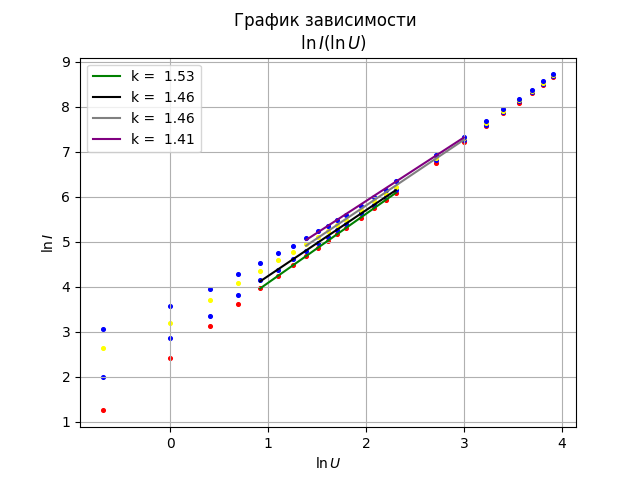
\includegraphics [scale=1.1]{lnI(lnU).png}}
		\caption{График зависимости $\ln I (\ln U)$}
	\end{figure}


	\newpage
	\item Используя данные, соответствующие участкам применимости «закона 3/2», построим для каждого тока накала вольт-амперные характеристики в координатах $I(U^{3/2})$.
	
	\begin{figure}[H]
		\center{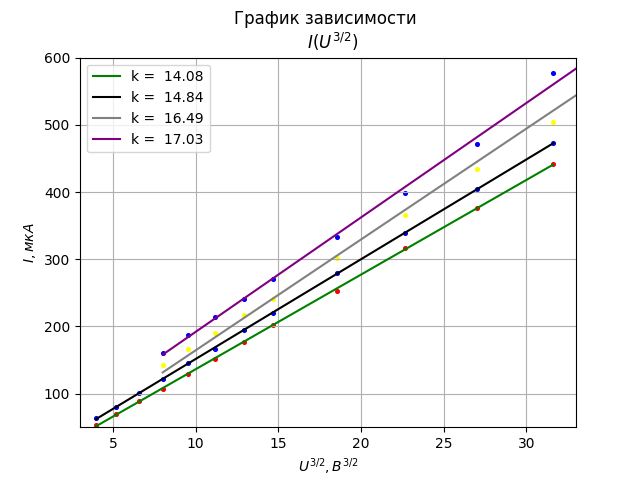
\includegraphics [scale=1.1]{I(U32).png}}
		\caption{График зависимости $I (U^{3/2})$}
	\end{figure}
	
	
	
	\item По полученным угловым коэффициентам определим удельную заряд электрона.
	
	$$ I = \sqrt{\dfrac{e}{m}} \dfrac{8\sqrt{2}\pi \varepsilon_0 l}{9}\dfrac{1}{r_a\beta^2} U^{3/2} = kU^{3/2}$$
	
	$$ \dfrac{e}{m} = k^2 \frac{81r_a^2\beta^4}{128\pi^2\varepsilon_0^2l^2} $$
	
	
	\end{enumerate}
	
	\begin{longtable} {|c|c|c|c|c|}
		\hline
		$I_H$,  А& 1,3 & 1,4 & 1,5 & 1,6   \\ \hline
		$ \frac{e}{m}, \cdot 10^{-11}$ Кл/кг & 1,67 & 1,84 & 2,28 & 2,42 \\ \hline
		\caption{Значения удельного заряда электрона при различных токах накала, $\sigma_{\frac{e}{m}} = 0,05 \cdot 10^{-11}$ Кл/кг}
	\end{longtable}
	
	
	\newpage
	
	\textbf{Выводы и обсуждение результатов}\\
	
	В данной работе мы определяли удельный заряд электрона на основе закона "трех вторых" для вакуумного диода. Мы получили, что закон выполняется при напряжениях не слишком маленьких и не слишком больших, объясняется это невозможностью пренебрежения начальными тепловыми скоростями электронов в первом случае и насыщением диода во втором. 
	
	Мы получили значения удельного заряда электрона близкие к табличному ($\frac{e}{m} = 1,76 \cdot 10^{-11}$ Кл/кг) только при токах 1,3 А и 1,4 А. Это можно объяснить тем, что мы снимали первые показания достаточно долго и ждали равновесия системы, а при токах 1,5 А и 1,6 А спешили записывать показания, что могло повлиять на результат.
	
	
	
	
	
	
	
	
	
	
	
	\end{document}